\chapter{The Schematic Editor}

CoolCAD Schematic Editor is the schematic capture tool for the CoolSPICE suite.  It comprises symbol and analysis tool libraries, symbol placement and wiring tools, and drawing tools with a built-in symbol editor for the design of new symbols.  The designer can create the SPICE netlist from the schematic and automatically invoke the CoolCAD SPICE engine to run the simulation from within the Schematic Editor.

Quick references to the tool buttons available in the Schematic Editor can be at the end of this Chapter.

\section{Drawing a Circuit}

By default, the Schematic Editor opens with an empty schematic named ``Cool1" in an inset window.  The inset windows can be closed, maximized to cover the full Schematic Editor ``desktop," or minimized.  A new window is opened by the \menuitem{File}{New}. An existing design is opened by the \menuitem{File}{Open...}.

\mymarginnote{Schematic \\navigation} The mouse scroll button can be used to zooming in or out of the schematic.  Clicking and holding the scroll button (or the middle button in a three-button mouse) can be used to pan around the schematic.

\subsection{Component Placement and Options}
\label{subsec_se_componentplacement}

Components are inserted by using the \textsf{Symbol Picker} frame, which is visible by default on the left-side of the Schematic Editor window and can be toggled on/off using the \menuorbutton{Symbol Picker} button (\fbox{$\Omega$}, see Fig. \ref{fig_schematiceditor_changePMOSwidth}).  The panel libraries can be expanded using the \fbox{+} buttons.  

Double-clicking a component name, or single-clicking and pressing the \makebutton{Place Symbol} button, or single-clicking the symbol representation in the frame underneath the library list, puts Schematic Editor in placing mode.  Multiple copies of a symbol can be placed by clicking consecutively in new locations.  

As with any action in the Schematic Editor, the placing action can be cancelled by pressing the \makekey{\textsc{Esc}} key.

Components are selected individually by clicking once on the symbol placed in the drawing area.  This brings the \window{Options} back up.  Figure \ref{fig_schematiceditor_annotatedoptions} shows the different elements of the \window{Options}:

\mymarginnote{Options\\details}
\begin{itemize}
\item \textit{Orientation Options} allow the user to place the symbol in four cardinal orientations and as a mirror-image if desired.
\item \textit{The Reference Name}, which may be automatically assigned by the program or manually by the user, is the name that the netlister will use to reference the component in the netlist.  Note that unclicking the tickbox next to \textsf{Ref} \textit{only hides the reference name in the circuit view}; the netlister still uses the reference name to identify the component.
\item \textit{Show Power Pins} enables/disables the display of power pins.
\item \textit{Allow Re-Sizing} shows or hides a resizing box with which the user can resize the symbol to better suit the design need.
\item \textit{The Temperature Setting} sets the individual device temperature for temperature-dependent parameter calculation during simulation.  This has no effect in the Student Edition.
\item \textit{The} \makebutton{Show Model} \textit{Button} shows the model card associated with the symbol.  If this model card is defined within a text file with an \textsf{.include} statement (see Section \ref{sec_se_symbolsandlibraries}) the program will display the entire file.
\item \textit{The Parameters} change depending on the component type.  Some parameters are compulsory to define for simulation.  More information on component parameters can be found for analysis commands and analysis-related components such as probes, and for active and passive devices as well as behavioral devices.
\item \textit{The} \makebutton{Add} \textit{and} \makebutton{Delete} \textit{Buttons} allow the user to define a new parameter or remove it. This is useful for user-defined symbols detailed in Section \ref{sec_se_symbolsandlibraries}.
\end{itemize}

\begin{SCfigure}[5.0][hbt]
    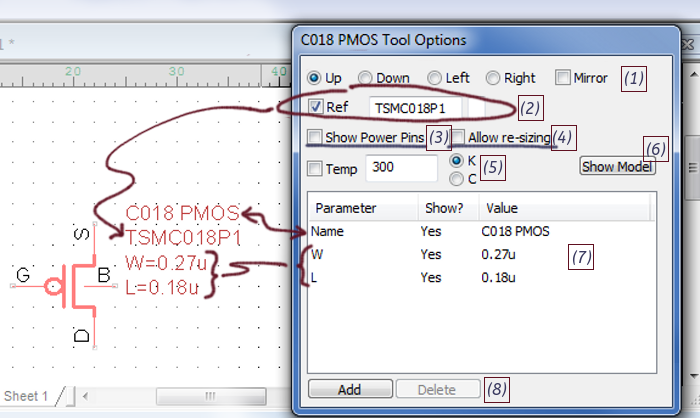
\includegraphics[width=0.65\textwidth]{./figures/schematic_editor_figures/SchematicEditor_PartOptionsDialogue_Annotated.png}
    \caption{{The Options window for a \textsf{TSMC 0.18um C018 PMOS} from the \textsf{MOSIS} library.  See the text body for the annotations.}}
  \label{fig_schematiceditor_annotatedoptions}
\end{SCfigure}


Right-clicking on the schematic window brings up a contextual menu which allows the user to perform some actions on the selected component, such as rotation, copy/paste, or cut.  The first option in the contextual menu, \textsf{Replace Symbol...} allows the user to replace either only the selected symbol, or all instances of this symbol in the design, by another symbol which must first be selected by entering part of its name into the search box.


\subsubsection{Reference Name Assignment}

The program automatically increments names for new instances of a given {component} if:
\begin{itemize}
\item The user picks the component by double-clicking on the name in the library or single-clicking on the symbol representation and places multiple instances by repeated clicks in the circuit design area without altering the \textsf{Ref} box in the \window{Options}, or
\item The user selects an already-placed component and chooses \menuitem{Edit}{Copy} / \menuitem{Edit}{Paste} (or uses the \makekey{Ctrl}-\makekey{C} / \makekey{Ctrl}-\makekey{V} key combinations) to place new instances without altering the \textsf{Ref} box in the \window{Options}.
\end{itemize}

\mymarginnote{Name\\increment\\exceptions}However, the software will \textit{not} increment the name in the case that the user:
\begin{itemize}
\item ...picks the component by double-clicking its name in the library list or single-clicking the symbol representation, and edits the reference name in the \textsf{Ref} box \textit{before} placing the first instance, or 
\item ...edits the reference name in the \textsf{Ref} box in between placing further instances, or
\item ...selects an already-placed component and edits the reference name in the \textsf{Ref} box to a name which contains only numbers (\textit{e.g.} ``123"), then uses the copy-paste method to make further copies.
\end{itemize}These cases may result in instances of the same component with identical names, which will lead to netlist conflicts. 

\inserttip{It is very important to ensure that each component instance has a distinct Reference Name.  Do not use reference names comprising only numbers.}

Also note that if the user edits the reference name of one of the instances of the same type of component to something out of the sequence, then makes further copies of the component, the incrementer will continue incrementing from the lowest available number appended.  For instance, if the circuit has instances \textsf{N1} through \textsf{N5}, and the user edits \textsf{N5} to \textsf{N42} and then places more instances by copy-pasting from any of the present instances, the incrementer will continue from \textsf{N5}, not \textsf{N43}.

\subsection{Wiring and Labels}
\label{subsec_se_wiringandlabels}

To start laying out a wire, click the \menuorbutton{Wire} tool button (see Fig. \ref{fig_schematiceditor_wiredtogether}) or press \makekey{F2}. The \window{Options} allows you to set the wire angle.  The first turn in the wire segment will be detected by the program depending on the mouse movement.  Double-clicking after a straight extension or right-clicking at any time ends the piece. When the wire crosses another wire, a circle appears to present the option of forming a connection with a single click.  A connection also ends the wire segment. Figure \ref{fig_schematiceditor_wiredtogether} shows the wired circuit just before the last connection is placed.

\mymarginnote{Labelling} In SPICE netlists, wires appear as the circuit nodes they represent.  If the wires are not labeled in the schematic, the netlister will use an automatic numbering scheme.  Labelling gives netlists that are easier to read (and after simulation, makes it easier to identify which signals to look at).  The \menuorbutton{Label} button (\fbox{\underline{a}}) or the \makekey{F1} key is used to set labels.  Figure \ref{fig_schematiceditor_labelexample} shows the net \textsf{Vout} being labelled.  In the \window{Label Options}, the top row is used to select the orientation of the letters.  The red dot that appears with the label on the schematic shows the location of the label (the net contacting this dot will take on the label).  Once the label is placed, the user can write another label name in the dialogue box.  The \makebutton{Font} and \makebutton{Colour} buttons can be used to set the font and color of the label on the schematic.

\begin{SCfigure}[5.0][hbt]
    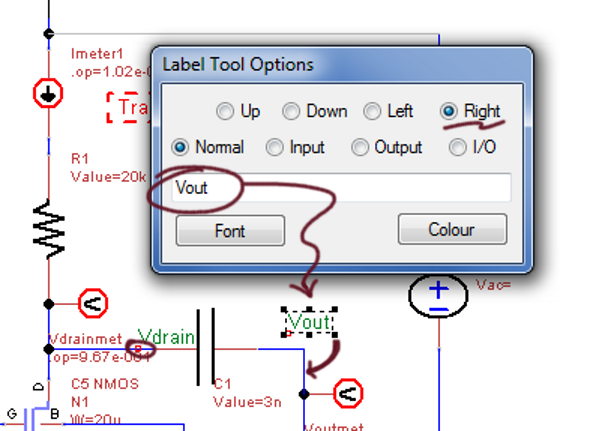
\includegraphics[width=0.65\textwidth]{./figures/schematic_editor_figures/SchematicEditor_LabelOptionsDialogue.png}
    \caption{{Labelling the node \textsf{Vout}.}}
  \label{fig_schematiceditor_labelexample}
\end{SCfigure}

With the labels, the MOSFET appears in the netlist with the following line:

\spicesyntax{\begin{tabular}{l}
MN1 Vdrain Vin Vs Vs on0p5nmos W=20u L=3u \\
\end{tabular} }

Whereas without the labels, the netlister automatically numbers the nodes:

\spicesyntax{\begin{tabular}{l}
MN1 \_N\_4 \_N\_8 \_N\_3 \_N\_3 on0p5nmos W=20u L=3u \\
\end{tabular} }

\subsection{Power Nets and Sources}
\label{subsec_se_powernetsandsources}

The power and ground nets are defined using inserted into the circuit using the \menuorbutton{Power} button (The "earth ground" symbol, see Fig. \ref{fig_schematiceditor_addVDD}) or pressing \makekey{F4}.  The name of the pin is entered using the dialogue box.   Different designs and orientations for the pin are available in the \window{Options}.

\inserttip{The ground pin name \textit{must} be \textbf{\texttt{0}}.} 

Multiple pins with the same name are used to denote the same node, which allows the user to avoid overly complicated wire networks in the schematic.  For an example, the netlist of the circuit shown in Fig. \ref{fig_schematiceditor_multiplepins} has the DC source \textsf{VS2} correctly wired between the away-from-drain end of the resistor \textsf{R1} and the ground.  For a circuit with multiple stages with drains all connected to \textsf{VDD}, this would cut down on the number of required wires.  This also enables multi-sheet designs, as described below in section \ref{sec_se_multisheetdesigns}.

\begin{SCfigure}[5.0][hbt]
    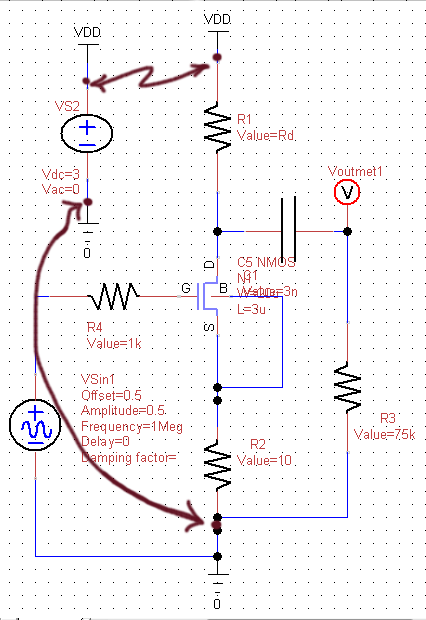
\includegraphics[width=0.4\textwidth]{./figures/schematic_editor_figures/SchematicEditor_MultiPinUseExample.png}
    \caption{{Using multiple copies of the same pin to clarify schematic design.  Each arrow-paired pair of marked dots are connected to the same node.}}
  \label{fig_schematiceditor_multiplepins}
\end{SCfigure}

\mymarginnote{Sources} The voltage and current sources are found under the \textsf{Analog} library.  The voltage sources are labeled ``\textsf{SourceV}" and current sources are labeled ``\textsf{SourceI}".  Details about the parameters of these components are found elsewhere. From the Schematic Editor the user can define DC/AC, Pulse (i.e. square wave) and Sinewave sources.  Other sources, such as the piecewise linear source, can be defined using the Netlist Editor.

\subsection{Probes}
\label{subsec_se_probes}

Inserting a current or voltage probe in the schematic directs the netlister to insert a \texttt{.save} statement in the netlist to store the branch current or node voltage results as appropriate for the proper analysis.  The probes are available in the Schematic Editor under the \textsf{Analog} library.  Naturally, current probes must be inserted into a branch and voltage probes connected to nodes.  Figure \ref{fig_transientsimexample} has an example circuit with a current probe measuring the drain current and three voltage probes measuring the gate, drain, and post-DC-filter output voltages.

\subsection{Further Navigation and Schematic Commands}
\label{subsec_se_morenavigation}

As mentioned above, one can use the mouse scroll button to zoom in and out of the design and the middle button/scroll button click-and-hold to pan around the circuit.  

Right-clicking anywhere around the drawing area brings up the contextual menu, which has a number of general commands and a number of selected-component-specific commands that are available.  (The selected-component-specific commands are greyed out unless the user right-clicks in the symbol area of a selected component.) Figure \ref{fig_schematiceditor_contextualmenu} shows the contextual menu invoked on the current meter \textsf{Imeter1} in the displayed circuit.

The \menuitem{Z-Order}{Bring to front} and \textbf{\textsf{Send to back}} commands in the contextual menu are useful for when images are imported into the Schematic Editor for use in a symbol or similar, as will be described in Section \ref{sec_se_hierarchicaldesigns}.  

It is possible to move the shown properties of components (including the reference names) to avoid conflicts and overlays.  In Figure \ref{fig_schematiceditor_contextualmenu} , the reference name \textsf{Voutmet1}, associated with the visible voltage probe, has been moved from its default location when the component is first set (which was directly above the visible \textsf{.op} line in the figure) by left-click and dragging on the text line.

\begin{SCfigure}[5.0][hbt]
    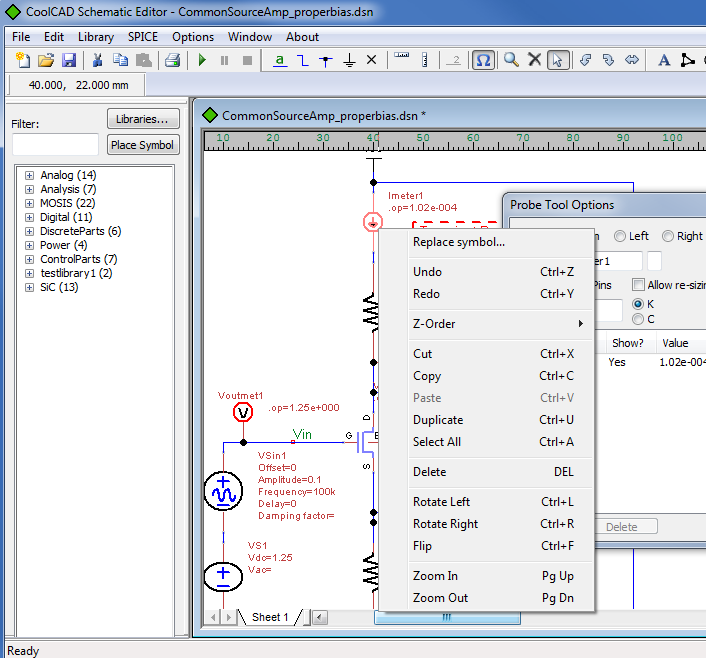
\includegraphics[width=0.6\textwidth]{./figures/schematic_editor_figures/SchematicEditor_ContextualMenu_MovingTextLabels.png}
    \caption{{The contextual menu comes up with a right-click in the schematic area.  If a device's symbol area is selected, the component-specific commands are enabled.  Also note that it is possible to move the reference name and property text for components, as for the case for the reference name of the voltage probe here.}}
  \label{fig_schematiceditor_contextualmenu}
\end{SCfigure}


\section{Multi-sheet Designs}
\label{sec_se_multisheetdesigns}

For complicated circuits, it is possible to split the circuit drawing into multiple sheets.  For a given design (\textsf{.dsn} file), the netlister will combine all sheets into a single circuit netlist.  Node and wire names should not be repeated between sheets except where a connection is explicitly intended, and the designer should take care that multiple components do not have the same reference name between sheets either.  

To start a new sheet, or to delete or rename a sheet, right click on the sheet tab at the bottom of the design window, which says \textsf{Sheet 1} by default when a circuit is first started.  

Use the power pins and wire labels to ensure correct connectivity between the circuit parts on different sheets.  For an example, Figure \ref{fig_schematiceditor_multisheetexample} shows a two-stage amplifier split into two sheets for illustration.  (While this is a circuit which could easily fit on a single sheet, the simplicity helps the example.)  The features to note here are how the drain-side voltage source for both transistors is defined on Sheet 1 as the voltage source \textsf{VS2} as described above in Section \ref{subsec_se_powernetsandsources}, how the gate, drain and source networks have distinguishing names between the two sheets, and how the DC-isolated output of stage 1, equivalently the DC-isolated input of stage 2, bears the same node name \textsf{Vout\_st1}. 

\begin{figure}[thb]
\centering
  \includegraphics[width=0.97\textwidth]
	{./figures/schematic_editor_figures/SchematicEditor_MultiSheetDesign.png}
  \caption{A two-stage amplifier as an example of multi-sheet design.}
  \label{fig_schematiceditor_multisheetexample}
\end{figure}

Part of the netlist for this circuit is shown here:

\spicesyntax{\begin{tabular}{l}
CC1 Vout\_st1 Vdrain\_st1 3n \\
CC2 Vout\_st2 Vdrain\_st2 3n \\
CC3 Vin\_st2 \_N\_13 3n \\
MN1 Vdrain\_st1 Vin\_st1 Vs1 Vs1 on0p5nmos W=20u L=3u \\ 
MN2 Vdrain\_st2 Vin\_st2 Vs2 Vs2 on0p5nmos W=20u L=3u \\
RR1 Vdrain\_st1 VDD 20k \\
RR10 \_N\_13 Vout\_st1 10 \\
(...) \\
RR4 0 Vout\_st1 75k \\
RR5 Vdrain\_st2 VDD 20k \\
(...) \\
RR7 0 Vout\_st2 75k \\
(...) \\
VVS2 VDD 0   DC  3  AC  0   \\
.save v(Vout\_st2) \\
.save v(Vout\_st1) \\
.save v(Vin\_st2) \\
.save v(Vin\_st1)
\end{tabular}}

% \spicesyntax{\begin{tabular}{l}
% * Schematics Netlist * \\
% .include "../Models/MyMOS.txt" \\
% \\ 
% MN1\_x line\_out \_HN\_1\_Vin 0 0 nmos0p5 W=3u L=0.6u \\
% MP1\_x line\_out \_HN\_1\_Vin \_HN\_1\_VDD \_HN\_1\_VDD pmos0p5 W=4.5u L=0.6u \\
% VVG1 \_HN\_1\_Vin 0   DC  3         \\
% VVS1 VDD 0   DC  3     \\
% \\
% .dc VVG1 0 3 0.05   \\
% .end 
% \end{tabular} }


Note that the resistors \texttt{RR1} and \texttt{RR5} are the resistors between the two transistors' drains and \textsf{VDD}, and they are correctly shorted to the same node whose voltage is set by the voltage source \texttt{VVS2}.  When this circuit is netlisted and ran, all the traces from the four visible voltage probes will be saved and be available for plotting.

\section{Models and Libraries}
\label{sec_se_symbolsandlibraries}

\subsection{Symbols and Hierarchical Designs}
\label{sec_se_hierarchicaldesigns}

\section{Netlisting and Simulation}
\label{sec_se_netlistingandsimulation}

\subsection{OP Analysis}
\label{sec_se_opanalysis}

\section{Options and Preferences}
\label{sec_se_optionsandpreferences}

\section{Schematic Editor GUI Reference}
\label{sec_se_guiref}

\newpage
\begin{figure}[h]
  \centering
    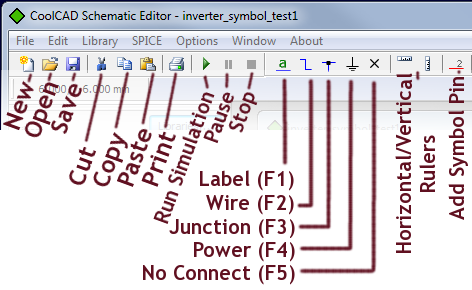
\includegraphics[width=0.72\textwidth]
		{./figures/appendix_buttons_menus_figures/SchematicEditor_LeftButtons.png}
    \caption{Left-side buttons on the Schematic Editor.}
  \label{fig_schematiceditor_leftbuttons_inchapter}
\end{figure} 

\vspace{\parskip}
\begin{figure}[htb]
  \centering
    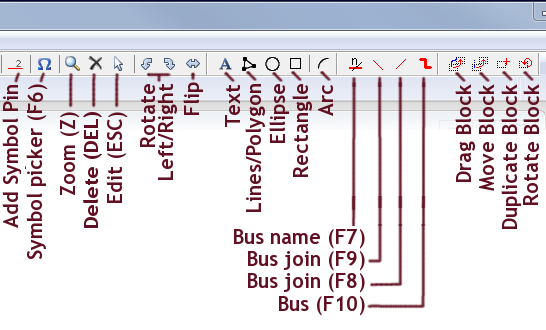
\includegraphics[width=0.72\textwidth]
		{./figures/appendix_buttons_menus_figures/SchematicEditor_RightButtons.png}
    \caption{Right-side buttons on the Schematic Editor.}
  \label{fig_schematiceditor_rightbuttons_inchapter}
\end{figure} 

A list of menu items for the Schematic Editor can be found in the Appendix.


